\section{Baseline Image-space Diffusion Pipeline}

The baseline model is trained directly on preprocessed two-dimensional RTI density fields. This pipeline is used as the reference against which the wavelet-based approach is compared.

The baseline pipeline follows the standard components of a score-based
generative model. The preprocessed RTI tensors are first loaded as
floating-point density fields and normalized to the interval $[-1,1]$. A
continuous variance-preserving SDE with affine $\beta(t)$ is then used to define
the forward noising process, the corresponding exact marginal perturbation, and
the probability-flow ODE used during sampling. The score network is a
time-conditioned U-Net trained to predict the target associated with the chosen
SGM parameterization, which is the $\mathbf{v}$-parameterization in the
baseline configuration.

During training, each batch is perturbed at a randomly sampled continuous
diffusion time. Gaussian noise is added according to the exact VP marginal, the
U-Net predicts the selected target, and the model parameters are updated by
minimizing the mean squared error between the true and predicted targets. A
validation set is used to monitor generalization and to retain the checkpoint
with the lowest validation loss for subsequent visualization and sampling.

The score network is a two-dimensional U-Net that receives a noisy density
field $\mathbf{x}_t$ together with the corresponding continuous diffusion time
$t$ and predicts the target required by the selected SGM parameterization. With
the $\mathbf{v}$-parameterization, the target is
\[
\mathbf{v}
=
\sqrt{\bar{\alpha}(t)}\,\boldsymbol{\epsilon}
-
\sqrt{1-\bar{\alpha}(t)}\,\mathbf{x}_0.
\]
The implementation then reconstructs
$\boldsymbol{\epsilon}_{\theta}(\mathbf{x}_t,t)$ from the network output and
converts it into a score estimate
$\mathbf{s}_{\theta}(\mathbf{x}_t,t)=-\boldsymbol{\epsilon}_{\theta}/\sigma(t)$.
This architecture is adapted to RTI fields because the encoder captures
large-scale organization whereas the decoder and skip connections preserve
localized structures near the mixing layer. In the implementation used here,
the input has shape $(1,64,64)$, the network contains three resolution levels,
and the timestep is encoded through a sinusoidal embedding injected at each
scale. The corresponding architecture is shown in Figure~\ref{fig:baseline_unet}.

\begin{figure}[H]
    \centering
    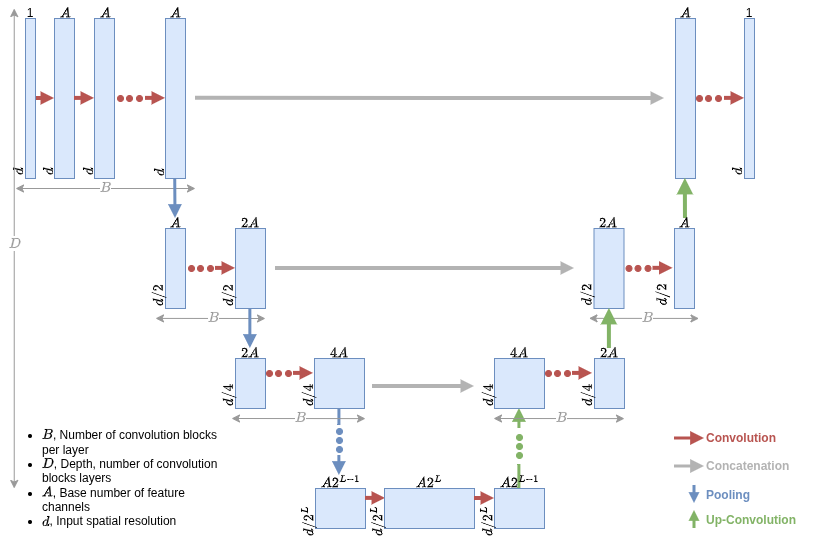
\includegraphics[width=0.82\textwidth]{figures/ch4/Unet2.drawio.png}
    \caption{Baseline U-Net score architecture used for image-space SGM. The noisy field is processed jointly with a continuous time embedding in order to predict the selected score-model target.}
    \label{fig:baseline_unet}
\end{figure}

At a high level, the baseline training procedure can be summarized as follows;
the same data flow is represented graphically in
Figure~\ref{fig:baseline_training_loop}.
\begin{algorithm}[H]
\caption{Baseline SGM training procedure}
\begin{algorithmic}
\STATE Load processed RTI density fields and build training and validation loaders.
\STATE Normalize each image to the interval $[-1,1]$.
\STATE Initialize an SGM with a time-conditioned U-Net and an affine VP-SDE noise schedule.
\FOR{each training epoch}
    \FOR{each batch $x_0$}
        \STATE Sample a continuous time $t\in[0,\mathds{1}]$ and Gaussian noise $\epsilon$.
        \STATE Compute $\bar{\alpha}(t)=\exp(-\int_0^t\beta(s)\,ds)$ and $\sigma(t)=\sqrt{1-\bar{\alpha}(t)}$.
        \STATE Build the noisy field $x_t=\sqrt{\bar{\alpha}(t)}x_0+\sigma(t)\epsilon$.
        \STATE Build the target $y_t=\epsilon$ for \texttt{epsilon}-prediction or $y_t=\sqrt{\bar{\alpha}(t)}\epsilon-\sigma(t)x_0$ for \texttt{v}-prediction.
        \STATE Predict $\hat{y}_\theta(x_t,t)$ with the U-Net.
        \STATE Minimize $\|y_t-\hat{y}_\theta(x_t,t)\|_2^2$.
    \ENDFOR
    \STATE Compute validation loss and save the checkpoint if it improves.
\ENDFOR
\end{algorithmic}
\end{algorithm}

Once the score network has been trained, generation is performed by starting
from a Gaussian prior at $t=\mathds{1}$ and integrating the deterministic
probability-flow ODE backward to a small terminal time
$\varepsilon_{\mathrm{time}}$. This is the deterministic counterpart of the
reverse SDE discussed in the score-based formulation and avoids injecting an
additional Brownian increment at every sampling step.

\begin{algorithm}[H]
\caption{Baseline SGM sampling procedure}
\begin{algorithmic}
\STATE Reload the best SGM checkpoint and set the U-Net to evaluation mode.
\STATE Sample $x_{\mathds{1}}\sim\mathcal{N}(0,I)$ with the target image shape.
\STATE Choose $N_{\mathrm{step}}$ integration steps, $\Delta t=-(\mathds{1}-\varepsilon_{\mathrm{time}})/N_{\mathrm{step}}$, and a solver, Heun by default.
\FOR{$i=0,\ldots,N_{\mathrm{step}}-1$}
    \STATE Set $t_i=\mathds{1}+i\Delta t$ and $t_{i+1}=t_i+\Delta t$.
    \STATE Reconstruct $\hat{\epsilon}_\theta(x_{t_i},t_i)$ from the network output.
    \STATE Compute the score
    $s_\theta(x_{t_i},t_i)=-\hat{\epsilon}_\theta(x_{t_i},t_i)/\sigma(t_i)$.
    \STATE Compute the probability-flow drift
    \[
        F_\theta(x_{t_i},t_i)
        =
        -\frac{1}{2}\beta(t_i)x_{t_i}
        -\frac{1}{2}\beta(t_i)s_\theta(x_{t_i},t_i).
    \]
    \STATE Predictor step: $\tilde{x}=x_{t_i}+\Delta t\,F_\theta(x_{t_i},t_i)$.
    \IF{Heun solver is used}
        \STATE Compute $F_\theta(\tilde{x},t_{i+1})$ and set
        \[
            x_{t_{i+1}}
            =
            x_{t_i}
            +
            \frac{\Delta t}{2}
            \left[
            F_\theta(x_{t_i},t_i)
            +
            F_\theta(\tilde{x},t_{i+1})
            \right].
        \]
    \ELSE
        \STATE Set $x_{t_{i+1}}=\tilde{x}$.
    \ENDIF
\ENDFOR
\STATE Clamp the final sample to $[-1,1]$.
\end{algorithmic}
\end{algorithm}

\begin{figure}[H]
    \centering
    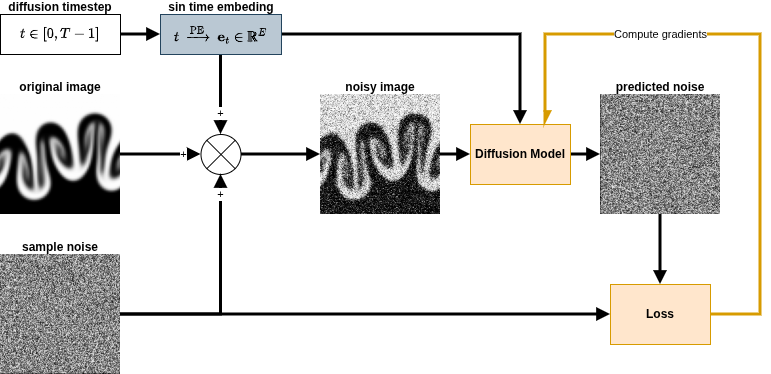
\includegraphics[width=0.82\textwidth]{figures/ch4/training_loop2.drawio.png}
    \caption{Baseline SGM training loop. A continuous diffusion time and Gaussian perturbation are sampled for each batch, and the U-Net is trained on the selected score-model target.}
    \label{fig:baseline_training_loop}
\end{figure}
